\documentclass[11pt]{article}
\usepackage[pdftex]{graphicx}
\usepackage{amsmath, amsthm, amssymb, amsfonts, mathtools, graphicx, enumerate}
\usepackage{times}
\usepackage{booktabs}
\usepackage{url}
\usepackage{color,soul}
\usepackage{enumerate}
\usepackage{listings}
%%\usepackage{enumitem}
\newcommand{\R}{\mathbb{R}}
\setlength{\parindent}{0pt}
\setlength{\parskip}{1ex}
\setlength{\oddsidemargin}{0.0in}
\setlength{\textwidth}{6.5in}
\setlength{\topmargin}{-0.5in}
\setlength{\textheight}{9.0in}
\newcommand{\RR}{\mathbb{R}}
\newcommand{\labelsymbol}{t}
\newcommand{\answer}[1]{{\mbox{}\color{red}{#1}}}
\newcommand{\emptycheck}{\text{(\hspace{-.75ex}(\hspace{3ex})\hspace{-.75ex})}}
\newcommand{\checkans}[1]{\text{(\hspace{-.75ex}(\hspace{1ex}{#1}\hspace{1ex})\hspace{-.75ex})}}
\newcommand{\argmax}{{\mbox{arg}\hspace{-.1ex}}\max}
\usepackage{hyperref}
\DeclarePairedDelimiter{\norm}{\lVert}{\rVert}
\title{EECS 498: Reinforcement Learning \protect \\ Homework 5 Responses}
\author{Tejas Jha \\ tjha}
\usepackage{amsmath}
\usepackage{verbatim}
\usepackage{enumitem}

\begin{document}

\maketitle
This document includes my responses to Homework 5 questions. Responses that involved the use of coding will provide references to specific lines of code to provide a better overview of how the problem was approached. The code can either be referenced in the Appendix or in the accompanied python script submitted with this assignment.

\section*{Question 1}
\begin{enumerate}[label=(\alph*)]
\item

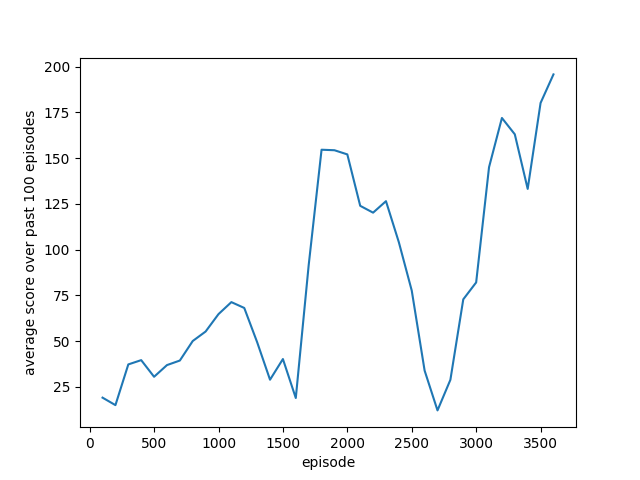
\includegraphics[scale=1]{testPole.png}

\item
To try and get the model working on MountainCar-v0, I first tried testing different values of C (which seemed to bring the peaks during training closer). I also tried testing different values for determining the decay rate of epsilon, (including latering the initial start point). If I had more time, I would attempt to adjust the some of the layers, with possibly including additonal ones to see how they perform.

\end{enumerate}
Suppose the reward function for an MDP is a linear function of d features for a state s

$$R(s) = \alpha_{1}\phi_{1}(s) + \alpha_{2}\phi_{2}(s) + ... +  \alpha_{d}\phi_{d}(s)$$

where the $\phi_{1} ... \phi_{d}$ are fixed, known and bounded basis functions mapping from state space $S$ to the reals. 

As presented in the Algorithms for Inverse Reinforcement Learning paper, we can define a value function for a policy $\pi$ that maps $S \mapsto A$  for any state $s_{1}$ as the following:

$$V^{\pi}(s_{1}) = E[R(s_{1}) + \gamma R(s_{2}) + \gamma^{2} R(s_{3}) + ... | \pi]$$

where the expectation is over the distribution of the state sequence $(s_{1}, s_{2}, ...)$.

Additionally from the same paper, we can use the notation $V_{i}^{\pi}$ to denote the value function of the policy $\pi$ in the MDP when the reward function is $R = \phi_{i}$. We can prove that for any policy $\pi$, the value function can be defined as $V^{\pi}(s_{1}) = \alpha_{1} V_{1}^{\pi} + \alpha_{2} V_{2}^{\pi} + ... + \alpha_{d} V_{d}^{\pi}$

We can substitute the reward function into the expectation in the value function equation and use the linearity of expectation to expand it to a sum of expectations of fixed and known values. There expectations would simplify to just the terms. This is shown below:

$$V^{\pi}(s_{1}) = E[R(s_{1}) + \gamma R(s_{2}) + \gamma^{2} R(s_{3}) + ... | \pi]$$
$$V^{\pi}(s_{1}) = E[\alpha_{1}\phi_{1}(s_{1}) + \alpha_{2}\phi_{2}(s_{1}) + ... +  \alpha_{d}\phi_{d}(s_{1})$$
$$ + \gamma * (\alpha_{2}\phi_{1}(s_{2}) + \alpha_{2}\phi_{2}(s_{2}) + ... +  \alpha_{d}\phi_{d}(s_{2})) +$$
$$ \gamma^{2}* (\alpha_{1}\phi_{1}(s_{3}) + \alpha_{2}\phi_{2}(s_{3}) + ... +  \alpha_{d}\phi_{d}(s_{3})) + ... | \pi]$$

$$V^{\pi}(s_{1}) = \alpha_{1}\phi_{1}(s_{1}) + \alpha_{2}\phi_{2}(s_{1}) + ... +  \alpha_{d}\phi_{d}(s_{1})$$
$$ + \gamma * (\alpha_{2}\phi_{1}(s_{2}) + \alpha_{2}\phi_{2}(s_{2}) + ... +  \alpha_{d}\phi_{d}(s_{2})) +$$
$$ \gamma^{2}* (\alpha_{1}\phi_{1}(s_{3}) + \alpha_{2}\phi_{2}(s_{3}) + ... +  \alpha_{d}\phi_{d}(s_{3})) + ... $$

The terms can now be regrouped using the alpha terms.

$$V^{\pi}(s_{1}) = \alpha_{1}*(\phi_{1}(s_{1}) + \gamma \phi_{1}(s_{2}) + \gamma^{2} \phi_{1}(s_{3}) + ... ) $$
$$
+ \alpha_{2}*(\phi_{2}(s_{1}) + \gamma \phi_{2}(s_{2}) + \gamma^{2} \phi_{2}(s_{3}) + ... )$$
$$
+ ... 
$$
$$
+ \alpha_{d}*(\phi_{d}(s_{1}) + \gamma \phi_{d}(s_{2}) + \gamma^{} \phi_{d}(s_{3}) + ... )
$$

$$V^{\pi}(s_{1}) = \alpha_{1}* E[\phi_{1}(s_{1}) + \gamma \phi_{1}(s_{2}) + \gamma^{2} \phi_{1}(s_{3}) + ... | \pi] $$
$$
+ \alpha_{2}*E[\phi_{2}(s_{1}) + \gamma \phi_{2}(s_{2}) + \gamma^{2} \phi_{2}(s_{3}) + ... | \pi]$$
$$
+ ... 
$$
$$
+ \alpha_{d}*E[\phi_{d}(s_{1}) + \gamma \phi_{d}(s_{2}) + \gamma^{2} \phi_{d}(s_{3}) + ... | \pi]
$$

Using the definition of $V_{i}^{\pi}$ and the equation for the value function, we can simplify the above expression to:

$$V^{\pi}(s_{1}) = \alpha_{1} V_{1}^{\pi} + \alpha_{2} V_{2}^{\pi} + ... + \alpha_{d} V_{d}^{\pi}
$$

Since $s_{1}$ is a variable to represent any arbitrary state, we can also just write the above as:

$$V^{\pi}(s) = \alpha_{1} V_{1}^{\pi} + \alpha_{2} V_{2}^{\pi} + ... + \alpha_{d} V_{d}^{\pi}
$$

This concludes the proof.

\section*{Question 2}


\section*{Appendix: Relevant Code - tjha\_hw5.py}
\lstinputlisting[language=Python, breaklines=true, numbers=left]{tjha_hw5.py}   
\end{document}
